\subsubsection{Modelo}

Pode-se ver nas figuras \ref{fig:C11} e \ref{fig:G1_11} o circuito e o gráfico, resp., do modelo de um motor de corrente contínua.

\begin{figure}[ht!]
\center
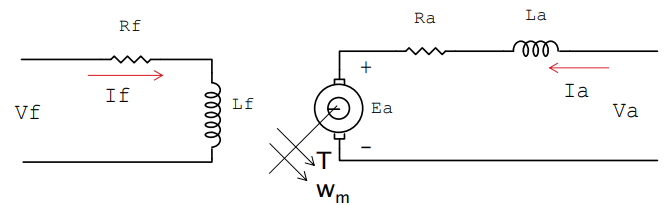
\includegraphics[scale=0.77]{imagens/circuito_11.png}
\caption{\label{fig:C11}Circuito elétrico do modelo geral.}
\caption*{Fonte: MARTINS, cap. 1, eslaide 4.}
\end{figure}

\begin{figure}[ht!]
\center
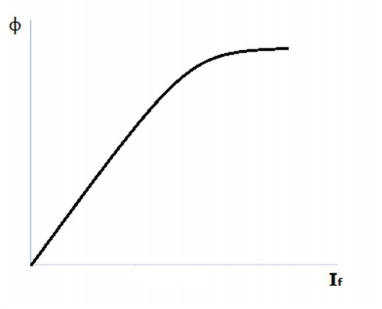
\includegraphics[scale=0.66]{imagens/grafico1_11.png}
\caption{\label{fig:G1_11}Curva de magnetização.}
\caption*{Fonte: MARTINS, cap. 1,  eslaide 4.}
\end{figure}

Partindo da curva de magnetização, podemos caracterizar completamente um motor CC através das equações

\[I_{f} = \frac{V_{f}}{R_{f}}\]

\[V_{a} = R_{a}I_{a} + E_{a}\]
\[E_{a} = k_{a}\phi{\omega_{m}}\]
\[T = k_{a}\phi I_{a}.\]

Assumindo que o motor opera na região linear, tem-se
\[\phi = k_{1}I_{f},\]
logo
\[E_{a} = k\omega_{m}I_{f}\]
\[T = kI_{f}I_{a}.\]

\subsubsection{Excitação separada constante e tensão de armadura variável}

Nesse caso, $\frac{\partial I_f}{\partial t} = 0$, logo

\[T = kI_{f}I_{a} = k_{2}I_{a}\]
\[E_{a} = k_{2}\omega_{m}\]
\[V_{a} = R_{a}I_{a} + E_{a} = R_{a}I_{a} + k_{2}\omega_{m}\]
\[\omega_{m} = \frac{V_{a} - R_{a}I_{a}}{k_{2}} = \frac{V_{a}}{k_{2}} - \frac{ R_{a}I_{a}}{k_{2}}.\]

Caso $R_{a} = 0$, $\omega_{m} = \frac{V_{a}}{k_{2}}$.

Diretamente, pode-se ver que a velocidade é diretamente proporcional à tensão de armadura. Entretanto, pela definição de $I_{f}$,

\[I_{a} = \frac{V_{a} - k_{2}\omega_{m}}{R_{a}},\]
logo,
\[T = \frac{k_{2}}{R_{a}}(V_{a} - k_{2}\omega_{m}) = \frac{k_{2}}{R_{a}}V_{a} - \frac{k_{2}}{R_{a}}k_{2}\omega_{m}.\]

Dessa forma, a velocidade do motor ($\omega_m$) pode ser estudada a partir da tensão de armadura (torque), como na figura \ref{fig:G1_12}. O circuito equivalente pode ser observado na figura \ref{fig:C12}.

\begin{figure}[ht!]
\center
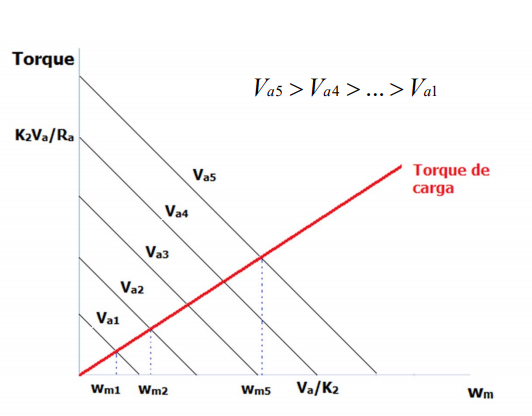
\includegraphics[scale=0.66]{imagens/grafico1_12.png}
\caption{\label{fig:G1_12}Curva Torque-Velocidade para o motor CC com excitação separada constante e tensão de armadura variável}
\caption*{Fonte: MARTINS, cap. 1, eslaide 7.}
\end{figure}


\begin{figure}[ht!]
\center
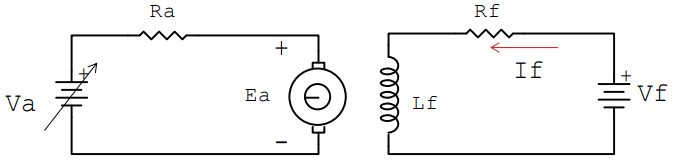
\includegraphics[scale=0.77]{imagens/circuito_12.png}
\caption{\label{fig:C12}Representação na forma de circuito}
\caption*{Fonte: MARTINS, cap. 1, eslaide 7.}
\end{figure}

As máquinas reais, entretanto, possuem $R_{a} \neq 0$, portanto as curvas comportam-se conforme ilustrado na figura \ref{fig:G2_12}.

\begin{figure}[ht!]
\center
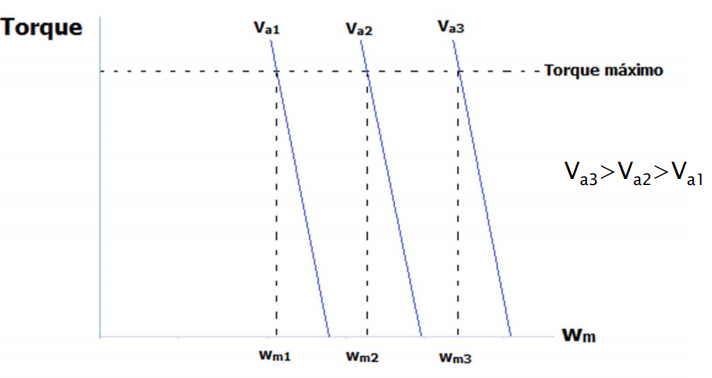
\includegraphics[scale=0.66]{imagens/grafico2_12.png}
\caption{\label{fig:G2_12}Torque em função da velocidade para $R_a \neq 0$}
\caption*{Fonte: MARTINS, cap. 1, eslaide 8.}
\end{figure}

Portanto, limitando $I_{a}$ podemos controlar o torque, uma vez que ele é proporcional à corrente de armadura.

\subsubsection{Excitação separada, corrente de armadura constante e corrente de campo variável}

Neste caso, muito útil quando se deseja motores mais compactos, o circuito é representado na figura \ref{fig:C13}.

\begin{figure}[ht!]
\center
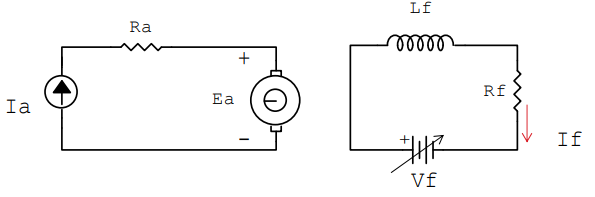
\includegraphics[scale=0.77]{imagens/circuito_13.png}
\caption{\label{fig:C13} Circuito equivalente do motor CC com excitação separada, corrente de armadura constante e corrente de campo variável.}
\caption*{Fonte: MARTINS,2006, eslaide 9.}
\end{figure}

Dado que $I_{a}$ é constante,
\[T = kI_{f}I_{a} = k_{4}I_{f}.\]

Vê-se que o torque não depende da velocidade. O comportamento do torque em função da velocidade é demonstrado na figura \ref{fig:G1_13}.

\begin{figure}[ht!]
\center
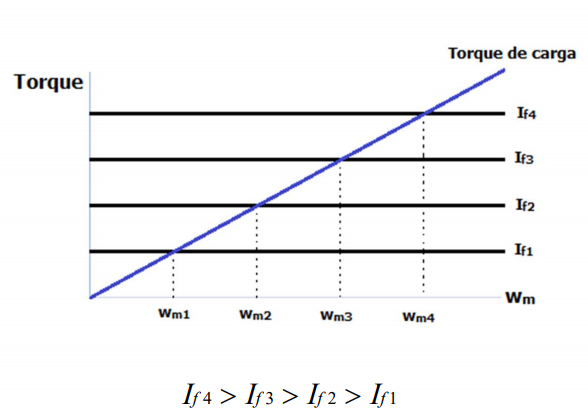
\includegraphics[scale=0.77]{imagens/grafico1_13.png}
\caption{\label{fig:G1_13}Curva Torque-Velocidade do motor CC em excitação separada, corrente de armadura constante e corrente de campo variável.}
\caption*{Fonte: MARTINS, cap. 1, eslaide 10.}
\end{figure}

Aqui, o conversor atua sobre a excitação onde a corrente é menor e a corrente de armadura é constante, o que impede que haja curto-circuito na armadura. Entretanto, o sistema é mais lento pois a constante de tempo mecânica é maior do que a elétrica.

\subsubsection{Excitação separada, tensão de armadura constante e corrente de campo variável}

Tomando como referência o circuito da figura \ref{fig:C14}, temos
\[E_{a} = k\omega_{m}I_{f} = V_{a} - R_{a}I_{a}\]
\[\omega_{m} = \frac{V_{a} - R_{a}I_{a}}{kI_{f}}.\]

\begin{figure}[ht!]
\center
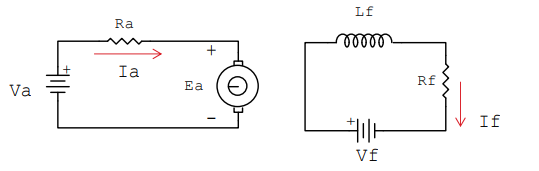
\includegraphics[scale=0.88]{imagens/circuito_14.png}
\caption{\label{fig:C14} Circuito equivalente do motor CC com excitação separada, tensão de armadura constante e corrente de campo variável.}
\caption*{Fonte: MARTINS, cap. 1, eslaide 11.}
\end{figure}

Supondo $R_{a} = 0$, $\omega_{m} = \frac{V_{a}}{kI_{f}} $. Dessa forma, ao atenuar o campo pode-se aumentar a velocidade, ou vice-versa.
\[T = kI_{f}I_{a} = kI_{f} \frac{(V_{a} - E_{a})}{R_{a}}\]
\[T = \frac{kV_{a}}{R_{a}}I_{f} - \frac{kI_{f}}{R_{a}}E_{a}\]
\[T = \frac{kV_{a}}{R_{a}}I_{f} - \frac{k^{2}I_{f}^{2}}{R_{a}}\omega_{m}.\]

I.e., o torque (T) se comporta como na figura \ref{fig:G1_14}.

\begin{figure}[ht!]
\center
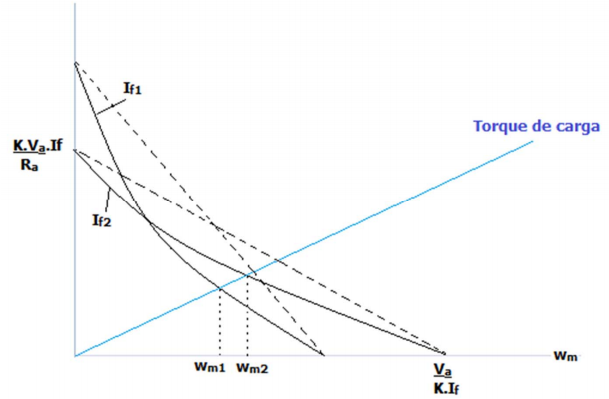
\includegraphics[scale=0.66]{imagens/grafico1_14.png}
\caption{\label{fig:G1_14} Curva Torque-Velocidade do motor CC com excitação separada, tensão de armadura constante e corrente de campo variável.}
\caption*{Fonte: MARTINS, cap. 1, eslaide 12.}
\end{figure}

Note que a diminuição da corrente $I_{f}$ provoca o aumento da velocidade do motor. 

\subsection{Excitação série}
 
A partir do circuito da figura \ref{fig:C15}, tem-se que $I_{f}=I_{a}$, portanto
\[E_{a} = kI_{f}\omega_{m} = kI_{a}\omega_{m}\]
\[V_{a} = R_{a}I_{a} + E_{a} = R_{a}I_{a} + k\omega_{m}I_{a}\]
\[I_{a} = \frac{V_{a}}{R_{a} + k\omega_{m}}\]
\[T = kI_{f}I_{a} = kI_{a}^{2} = \frac{kV_{a}^{2}}{(R_{a} + k\omega_{m})^{2}}.\]
 
\begin{figure}[ht!]
\center
\caption{\label{fig:C15} Circuito equivalente do motor CC com excitação série.}
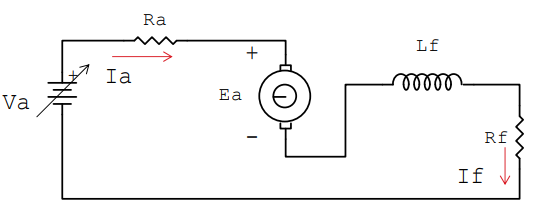
\includegraphics[scale=0.77]{imagens/circuito_15.png}
\caption*{Fonte: MARTINS, cap. 1, eslaide 13.}
\end{figure}


Se $R_{a} = 0$,
\[T = \frac{V_{a}^{2}}{k\omega_{m}^{2}}.\]

A relação torque-velocidade encontra-se representado graficamente na figura \ref{fig:G1_15} para diferentes valores de $V_{a}$.

\begin{figure}[t!]
\center
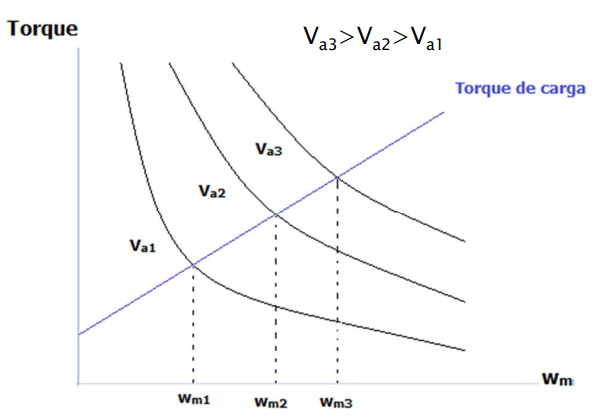
\includegraphics[scale=0.66]{imagens/grafico1_15.png}
\caption{\label{fig:G1_15}Curva Torque-Velocidade do motor CC com excitação série.}
\caption*{Fonte: MARTINS, cap. 1, eslaide 14.}
\end{figure}
 
É possível controlar a velocidade através da variação da tensão de alimentação de armadura.

O motor série oferece, principalmente, um elevado torque de partida. Por isso, ele é tipicamente utilizado em aplicações que necessitam de tração elétrica, além de aplicações de baixa potência.
